%%%%%%%%%%%%%%%%%%%%%%%%%%%%%%%%%%%%%
%%%%%%%%%%%%%%%%%%%%%%%%%%%%%%%%%%%%%
%
%   Hi, All
%   Arun Xavier, VAST Thrissur
%
%   for more  Visit my Page - http://arunxeee.blogspot.in/
%
%%%%%%%%%%%%%%%%%%%%%%%%%%%%%%%%%%%%
%%%%%%%%%%%%%%%%%%%%%%%%%%%%%%%%%%%%

%%
\documentclass[12 pt, oneside]{book}
\usepackage{graphicx, fancyhdr, amsmath, times, enumerate,geometry,makeidx,setspace,nomencl,eso-pic,xcolor,lipsum,calc,pst-node,tikz,fancybox,background,caption,subcaption,amsfonts}




\usetikzlibrary{calc}
\SetBgScale{1}
\SetBgAngle{0}
\SetBgColor{brown}
\SetBgOpacity{1}
%%
\geometry{verbose,a4paper,tmargin=1 in,bmargin=1in,lmargin=1.5 in,rmargin=.9 in}
%%%%%%%%%%%%%%%%%%%%%%%%%%%%%%%

\makeindex

%%
\usepackage[final]{pdfpages}
%%
%\setlength{\oddsidemargin}{2 cm}



%%
\newcommand{\VAtitle}[1]%
{\def\vtitle{#1}}%
\newcommand{\VAauthora}[1]%
{\def\vauthora{#1}}%
\newcommand{\VAauthorb}[1]%
{\def\vauthorb{#1}}%
\newcommand{\VAauthorc}[1]%
{\def\vauthorc{#1}}%
\newcommand{\VAauthord}[1]%
{\def\vauthord{#1}}%
\newcommand{\VAauthore}[1]%
{\def\vauthore{#1}}%
\newcommand{\VAadmissionyear}[1]%
{\def\vadmissionyear{#1}}%
\newcommand{\VAacademicyear}[1]%
{\def\vacademicyear{#1}}%
\newcommand{\VAprincipal}[1]%
{\def\vprincipal{#1}}%
\newcommand{\VAguide}[1]%
{\def\vguide{#1}}%
\newcommand{\VAguidedg}[1]%
{\def\vguidedg{#1}}%
\newcommand{\VAhod}[1]%
{\def\vhod{#1}}%
\newcommand{\VAdate}[1]%
{\def\vdate{#1}}%
\newcommand{\VAdept}[1]%
{\def\vdept{#1}}%
\newcommand{\VAclass}[1]%
{\def\vclass{#1}}%
\newcommand{\VApaper}[1]%
{\def\vpaper{#1}}%
%%
%%



\SetBgContents{}



\VApaper{DESIGN PROJECT REPORT}

\usepackage{titlesec}
\titleformat{\chapter}[display]
{\normalfont\LARGE\bfseries\centering}{\chaptertitlename\ \thechapter}{20pt}{\Huge}

\begin{document}
	\VAtitle{PRODUCT STUDY AND DESIGN}
\VAauthora{SEBASTIAN T F (VAS16CS102)}
\VAauthorb{SHABANA P J (VAS16CS103)}
\VAauthorc{SHAHEEN N S (VAS16CS104)}
\VAadmissionyear{2016}
\VAprincipal{Dr. Saji C.B}
\VAguide{Ms. Aswathy M.R}
\VAguidedg{Asst. Prof.,}
\VAhod{Dr. Ramani Bai V}
\VAdate{November 2018}
\VAacademicyear{2018-2019}
\VAdept{Computer Science \&  Engineering}
\VAclass{B.Tech (CSE)}

\pagestyle{empty}
%%%%%%%%%%%%%%%%%%%%%%%%%%%%%%%%%%%%%
%%%%%%%%%%%%%%%%%%%%%%%%%%%%%%%%%%%%%
%
%   Hi, All
%   Arun Xavier, VAST Thrissur
%
%   for more  Visit my Page - http://arunxeee.blogspot.in/
%
%%%%%%%%%%%%%%%%%%%%%%%%%%%%%%%%%%%%
%%%%%%%%%%%%%%%%%%%%%%%%%%%%%%%%%%%%
%
%******************************************************
%

\begin{spacing}{1.5}
\begin{titlepage}




\SetBgContents{

\begin{tikzpicture}[overlay,remember picture]
\draw [line width=3pt]
    ($ (current page.north west) + (3.0cm,-1.8cm) $)
    rectangle
    ($ (current page.south east) + (-1.35cm,1.8cm) $);
\draw [line width=1pt]
    ($ (current page.north west) + (3.15cm,-1.95cm) $)
    rectangle
    ($ (current page.south east) + (-1.5cm,1.95cm) $); 
\end{tikzpicture}
}

\begin{center}

\vspace{1 cm}

{ \LARGE \rmfamily \bf \vtitle}\\[1 cm]

{ \large \rmfamily A \vpaper \\ SUBMITTED IN PARTIAL FULFILLMENT OF THE \\REQUIREMENTS FOR THE AWARD OF DEGREE OF}\\[1 cm]

{ \Large \rmfamily \bf BACHELOR OF TECHNOLOGY}\\
{\large \rmfamily in}\\[.2 cm]
{ \Large \rmfamily \bf COMPUTER SCIENCE AND ENGINEERING}\\
{\large \rmfamily of}\\[.2 cm]
{ \Large \rmfamily \bf APJ ABDUL KALAM TECHNOLOGICAL UNIVERSITY}\\
{\large \rmfamily by}\\[.4 cm]
{\large \rmfamily \bf \vauthora }\\
{\large \rmfamily \bf \vauthorb } \\
{\large \rmfamily \bf \vauthorc } \\[1.5 cm]
%

%

\includegraphics[width=3.5 cm]
{VidyaLogo.jpg}\\
\scriptsize (AN ISO 9001:2008 CERTIFIED INSTITUTION )\\[1.5 cm]

%
{\Large \bf Department of \vdept}\\
{\Large \rmfamily Vidya Academy of Science \& Technology\\[.2 cm]
\large Thalakkottukara, Thrissur - 680 501}\\
({ \bf \tt http://www.vidyaacademy.ac.in})\\[.4 cm]
{\large \rmfamily \vdate}


\end{center}
\end{titlepage}
%
%******************************************************
%
\clearpage


\pagenumbering{gobble}
%\pagestyle{empty}
\addcontentsline{toc}{chapter}{\quad CERTIFICATE}




\begin{titlepage}
\SetBgContents{

\begin{tikzpicture}[overlay,remember picture]
\draw [line width=3pt]
    ($ (current page.north west) + (3 cm,-1.8cm) $)
    rectangle
    ($ (current page.south east) + (-1.5cm,1.8cm) $);
\draw [line width=1pt]
    ($ (current page.north west) + (3.15cm,-1.95cm) $)
    rectangle
    ($ (current page.south east) + (-1.65cm,1.95cm) $); 
\end{tikzpicture}
}


\begin{center}


{\Large \bf Department of \vdept  }\\
{\Large \bf Vidya Academy of Science \& Technology}\\
{\normalsize \bf Thalakkottukara, Thrissur - 680 501\\
({\tt http://www.vidyaacademy.ac.in})}\\[0.75cm]
%
%   Logo
%

\includegraphics[width=3.5 cm]{VidyaLogo.JPG}\\
\scriptsize (AN ISO 9001:2008 CERTIFIED INSTITUTION )\\[1 cm]
%
 \Huge  $ \mathfrak{Certificate}$\\[0.5cm]
%
\end{center}
\index{Certificate}
\index{University of Calicut}

\quad This is to certify that the Design Project Report titled {\bf ``\vtitle"} is a bonafide record of the work carried out by {\bf \vauthora\, \vauthorb\, \vauthorc } of Vidya Academy of Science \& Technology, Thalakkottukara, Thrissur - 680 501 in partial fulfillment of the requirements for the award of  {\bf Degree of Bachelor of Technology} in {\bf Computer Science and Engineering} of  {\bf APJ Abdul Kalam Kerala Technological University, Kerala}, during the academic year \vacademicyear. The Design Project report has been approved as it satisfies the academic requirements in the respect of Design Project work prescribed for the said degree.\\[1 cm]
 
\noindent{\bf Project Guide/Supervisor} \hfill  {\bf Head of Department} \\[.3cm]
\noindent \vguide \hfill \vhod \\ \vguidedg\ Dept. of CSE \hfill Dept. of CSE \\
Sig:...............  \hfill  Sig:............... \\[.25 cm]
\noindent Ms. Remya P.S\\
\vguidedg\, Dept. of CSE \\
Sig:............... 




%
\end{titlepage}

%   End of Certificate
%  
\clearpage


%   Redefining plain page style
%  
\fancypagestyle{plain}{%
\fancyhf{} % clear all header and footer fields
\fancyhead[L]{{\scriptsize \vtitle}}
\fancyhead[R]{
\includegraphics[width=0.5cm]{VidyaLogo.JPG}}
%\fancyfoot[C]{\bfseries \thepage} 
\fancyfoot[L]{{\footnotesize Department of Computer Science \&  Engg.}}
\fancyfoot[R]{\footnotesize VAST, Thalakotukara}
\fancyfoot[C]{\footnotesize \bf \thepage}%
\renewcommand{\headrulewidth}{1pt}%
\renewcommand{\footrulewidth}{1pt}%
}%
%

\pagenumbering{roman}

\pagestyle{plain}
\addcontentsline{toc}{chapter}{\quad ACKNOWLEDGEMENT}
%%%%%%%%%%%%%%%%%%%%%%%%%%%%%%%%%%%%%
%%%%%%%%%%%%%%%%%%%%%%%%%%%%%%%%%%%%%
%
%   Hi, All
%   Arun Xavier, VAST Thrissur
%
%   for more  Visit my Page - http://arunxeee.blogspot.in/
%
%%%%%%%%%%%%%%%%%%%%%%%%%%%%%%%%%%%%
%%%%%%%%%%%%%%%%%%%%%%%%%%%%%%%%%%%%


%
\chapter*{\centering Acknowledgement}
%


\par
\hspace{0.9cm}
\vspace {.2cm}
\par
\hspace{.35cm}I would like to thank the Lord Almighty, the foundation of all wisdom who has been guiding us in every step. I wish to record my indebtedness and thankfulness to all who helped me to prepare this design project titled {\bf \vtitle} and present it in a satisfactory way. This report is part of my work related to the paper CS 341 DESIGN PROJECT 
\vspace{0.2cm}
\par
\hspace{0.35cm}My sincere thanks to {\bf \vprincipal}, Principal, for providing me all the necessary facilities. I take this opportunity to extend my thanks to {\bf \vhod} the Head of {\bf \vdept} for giving me valuable guidance in developing this project. I'm extremely thankful to my guides and supervisors {\bf \vguide}, Asst.Professor, {\bf Ms. Remya P.S}, Asst.Professor in the Department of {\bf \vdept} for giving me valuable suggestions and critical inputs in the preparation of this report. 
\vspace{.2cm}
\par 
\hspace{.35cm}I express my heartfelt thanks to the {\bf Lab Instructors} for their valuable support and assistance for my work. My sincere thanks to {\bf parents and friends} who have helped me during the course of the project work and made it a great success.

\begin{flushright}
{\vauthora}\\
{\vauthorb}\\
{\vauthorc}

\vclass\  (\vadmissionyear\  Admissions)\\
Vidya Academy of Science \& Technology\\
\vdate  \hfill Thrissur - 680 501.
\end{flushright}








\chapter*{\centering{Abstract}}
\addcontentsline{toc}{chapter}{\quad ABSTRACT}
\hspace{0.1cm}{\bf Study} :- Several solutions exist today that provide platforms to learn coding. Online courses are revolutionizing such education. Such courses deliver a series of lessons on a web browser or mobile device, to be coveniently accessed any time, any place. Many online courses are available today to learn coding. In this paper, we collected data about some popular platforms that provide online coding lessons. By this study we were able to recognize the downsides and advantages of these platforms and come up with a better solution than existing ones.\\\\
{\bf Codecademy} \\
Codecademy is an online interactive platform that offers free coding classes in several programming languages. It is a site where you get introduced to programming whilst doing it real-time.\\
{\bf Udemy} \\
Udemy is a global marketplace for learning and teaching online where students are mastering new skills and achieving their goals by learning from an extensive library of over 80,000 courses taught by expert instructors. \\
{\bf Dialogflow} \\
Dialogflow is a chatbot platform provided by Google. It enables us to develop and implement a chatbot within our products. It provides a great experience in Natural Language Processing and can be integrated with a wide range of apps and services.\\\\
{\bf Design :- Virtua Teacher} \\
Virtua Teacher is an integration of Data Analysis and Intelligence to the existing online learning platforms so that it can achieve the ability to enable in-depth training and more interactivity.


%%%%%%%%%%%%%%%%%%%%%%%%%%%%%%%%%%%%
%%%%%%%%%%%%%%%%%%%%%%%%%%%%%%%%%%%%
%       
%		Do not change any thing after this . . .
%
%%%%%%%%%%%%%%%%%%%%%%%%%%%%%%%%%%%%
%%%%%%%%%%%%%%%%%%%%%%%%%%%%%%%%%%%%
\tableofcontents
\addcontentsline{toc}{chapter}{\quad  LIST OF FIGURES}
\listoffigures
% For adding List of symbols or abbreviations
\addcontentsline{toc}{chapter}{\quad  LIST OF SYMBOLS AND ABBREVIATIONS}
%%%%%%%%%%%%%%%%%%%%%%%%%%%%%%%%%%%%%
%%%%%%%%%%%%%%%%%%%%%%%%%%%%%%%%%%%%%
%
%   Hi, All
%   Arun Xavier, VAST Thrissur
%
%   for more  Visit my Page - http://arunxeee.blogspot.in/
%
%%%%%%%%%%%%%%%%%%%%%%%%%%%%%%%%%%%%
%%%%%%%%%%%%%%%%%%%%%%%%%%%%%%%%%%%%
%
%
%



\chapter*{List of Symbols and Abbreviations}




\begin{tabbing}



\hspace{1cm}\= {$ \bf VAST   $}\quad\= - Vidya Academy of Science and Technology\\[5pt]

\hspace{1cm}\= {$ \bf I/O  $}\quad\= - Google Annual Developer Conference\\[5pt]
\hspace{1cm}\= {$ \bf AI  $}\quad\= - Artificial Intelligence\\[5pt]
\hspace{1cm}\= {$ \bf ML   $}\quad\= - Machine Learning \\[5pt]
\hspace{1cm}\= {$ \bf DL    $}\quad\= - Deep Learning \\[5pt]
\hspace{1cm}\= {$ \bf PDF    $}\quad\= - Portable Document Format\\[5pt]
\hspace{1cm}\= {$ \bf GPS    $}\quad\= - Global Positioning System\\[5pt]
\hspace{1cm}\= {$ \bf SDLC   $}\quad\= - System Development Life Cycle\\[5pt]
\hspace{1cm}\= {$ \bf SRS    $}\quad\= - Software Requirement Specification\\[5pt]
\hspace{1cm}\= {$ \bf DDS    $}\quad\= - Design Document Specification\\[5pt]
\hspace{1cm}\= {$ \bf DFD    $}\quad\= - Data Flow Diagram\\[5pt]
\hspace{1cm}\= {$ \bf UML    $}\quad\= - Unified Modeling Language\\[5pt]
\hspace{1cm}\= {$ \bf UI     $}\quad\= - User Interface\\[5pt]
\hspace{1cm}\= {$ \bf UX     $}\quad\= - User Experience\\[5pt]

\end{tabbing}
\mainmatter



\chapter {PRODUCT STUDY}
\section {Codecademy}
{\em Codecademy is an online interactive platform that offers free coding classes in several programming languages. It also provide classes and lessons on many other skills related to software development and coding.}

\subsection{Introduction}    % For giving Section  eg: 1.1

Codecademy is an online interactive platform that offers free coding classes in 12 different programming languages including Python, Java, JavaScript (jQuery, AngularJS, React.js), Ruby, SQL, and Sass, as well as markup languages HTML and CSS. The site also offers a paid "pro" option that gives users access to a personalized learning plan, quizzes, realistic projects, and live help from advisors.

\begin{figure}[h]
	\label{ss}    %Figure Label is used
	\centering
	
\includegraphics[width= 5 cm]{logo.jpeg}
	\caption{Codecademy}
\end{figure}



% You can add any sections like that . . . 

\subsection{Features }

Codecademy has a lot of features built into it which makes it one of top best methods to learn coding. It is a really rich and robust web application. From design to functionality and the lessons it provides, it is a well developed and maintained application which requires a lot of work to be put into.


  %\ref for the figure label, check the below figure.

%%%%%%%%%%%%%%%%%%%%%%%%%%%%%%%%%%%
%		Before using image put the jpg image file in the folder. 
%		Here   ct.jpg   is the file name
%%%%%%%%%%%%%%%%%%%%%%%%%%%%%%%%%%%
\subsubsection {Dashboard}
The dashboard is what the user is presented with right after the user logs into his/her account in Codecademy. Codecademy has a really well designed dashboard which looks modern. The dashboard displays much of the information of the user's courses. It shows the course that was last attended by the user, shows how much of the course has been completed and provides an option to resume the course. Dashboard also provides options to select a new path or level of learning. All the courses enrolled by the user are viewable in the dashboad\\

\begin{figure}[h]
	\label{ss}    %Figure Label is used
	\centering
	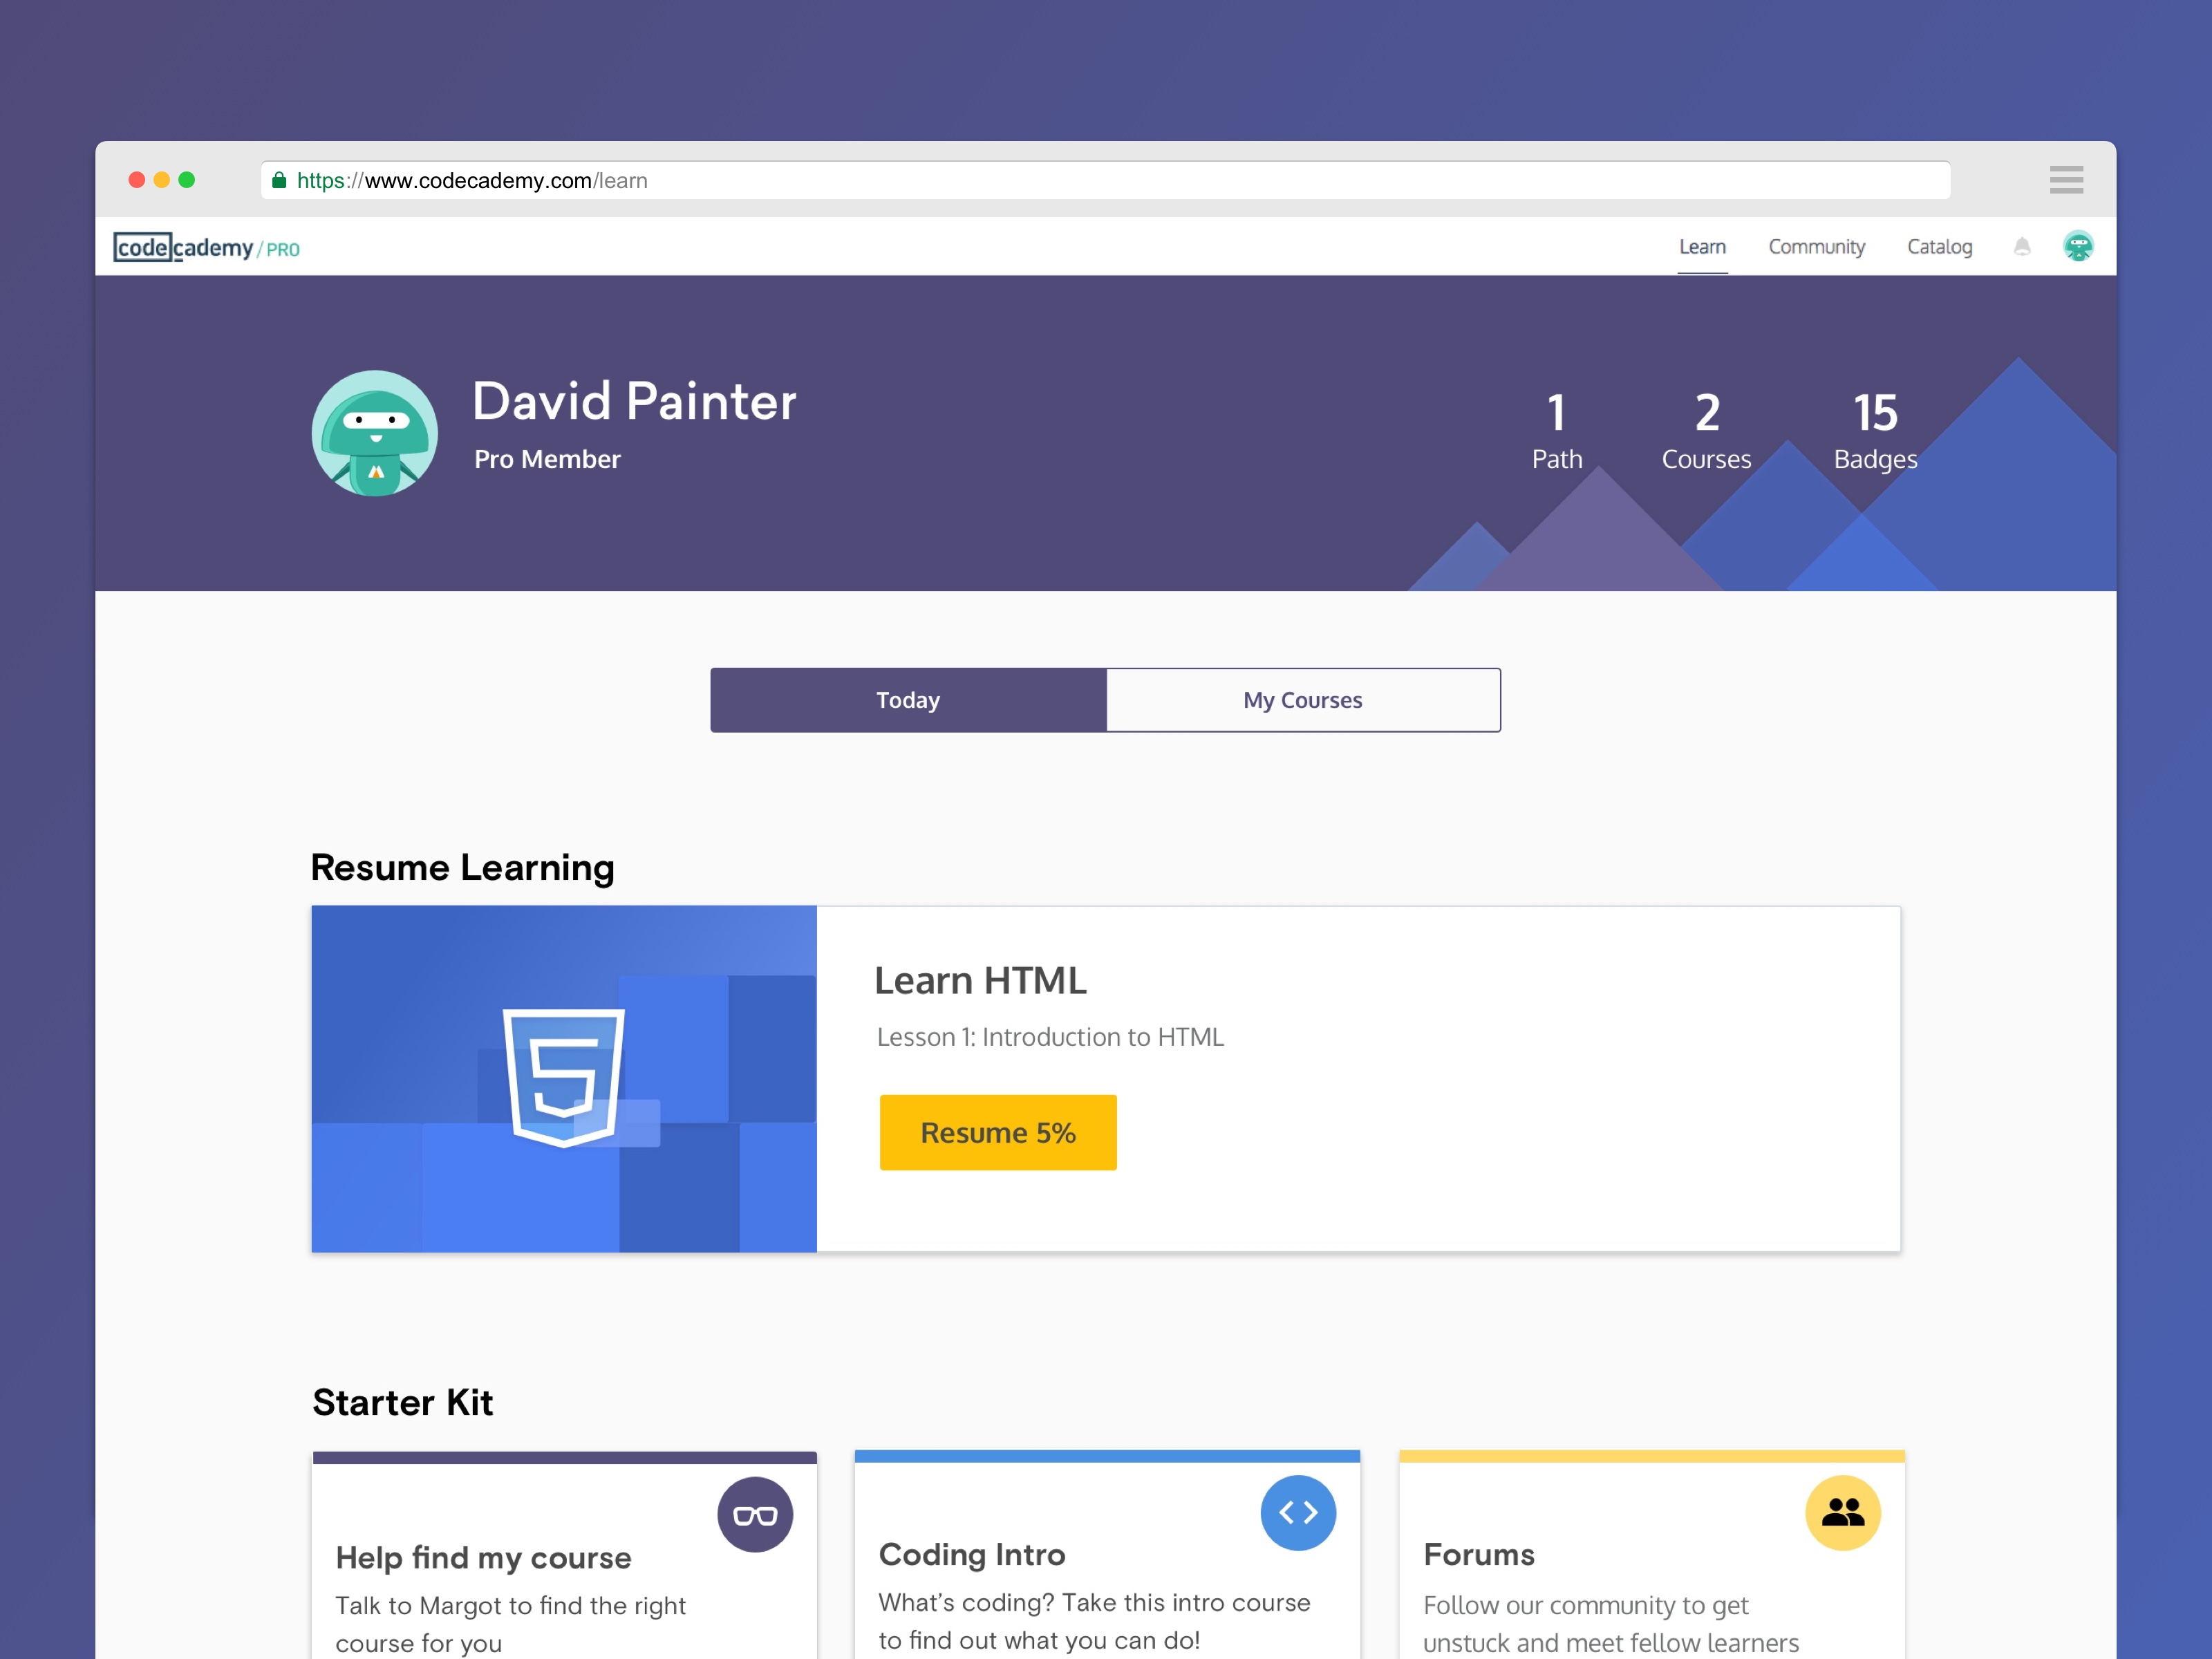
\includegraphics[width= 15 cm,height=10 cm]{dashboard.jpg}
	\caption{Dashboard}
\end{figure}

\newpage
\begin{figure}[h]
	\label{ss}    %Figure Label is used
	\centering
	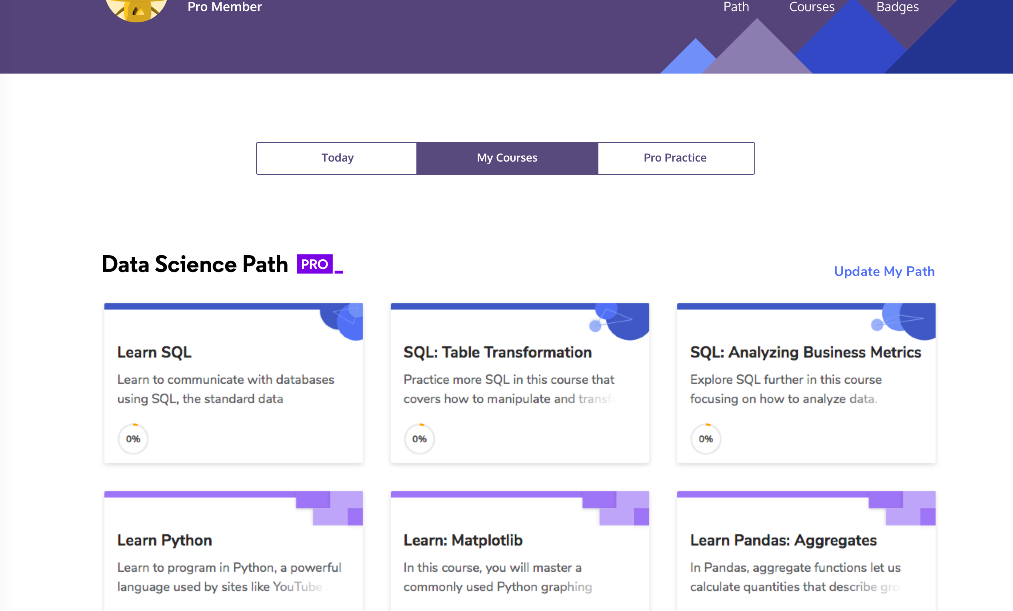
\includegraphics[width= 15 cm, height=10cm]{mycourses.png}
	\caption{My Courses}
\end{figure}

\subsubsection {Course Catalog}
Codecademy offers a wide range of courses. All the courses offered at Codecademy can be viewed in the Course Catalog which is really huge. Codecademy is nothing if not prolific, and one of their best features is just the breadth of their offerings. To date they have tutorials on HTML, CSS, Sass, JavaScript, Rails, AngularJS, ReactJS, Ruby, Command Line, Git, SQL, and Java. They offer 48 courses, 13 Intensive Programs and 4 Paths which is a lot of courses and resources to learn.

\begin{figure}[h]
	\label{ss}    %Figure Label is used
	\centering
	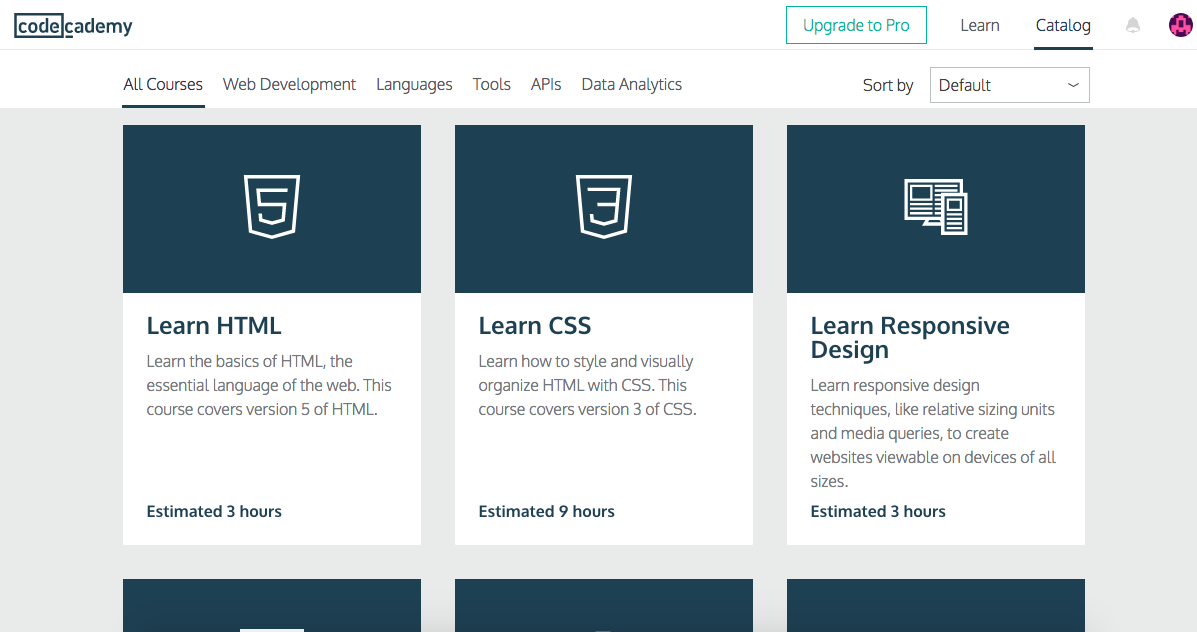
\includegraphics[width= 10 cm]{coursecatalog.png}
	\caption{Courses Catalog}
\end{figure}

\subsubsection {Online IDE}
Codecademy has developed a web-based code editor called 'Labs'. It can be used to practice the code that we've learned in various courses while learning each lesson without having to download a desktop-based code editor or integrated development environment (IDE). The interactive coding console allows you to program in all the languages being taught at Codecademy as a way to practice languages and implement curriculum you may have learned elsewhere.

\begin{figure}[h]
\label{ss}    %Figure Label is used
\centering
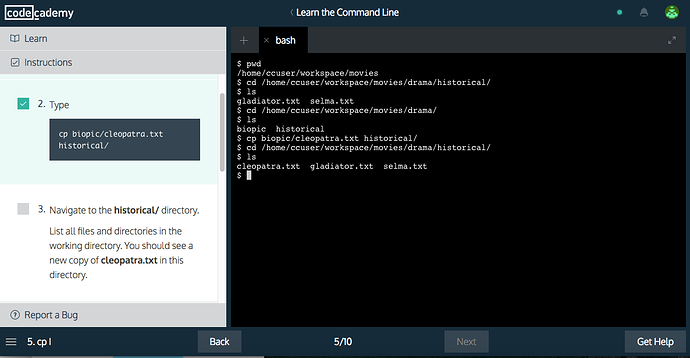
\includegraphics[width= 15 cm,height=10cm]{ide.jpg}
\caption{Built-in Online IDE}
\end{figure}

\subsection{History}

Codecademy was founded in August 2011 by Zach Sims and Ryan Bubinski. Sims dropped out of Columbia University to focus on launching a venture, and Bubinski graduated from Columbia in 2011. The company, headquartered in New York City, raised \$2.5 million in Series A funding in October 2011 and \$10 million in Series B funding in June 2012. The latest round of funding was led by Index Ventures. Crunchbase reports an additional Series C round of funding for an undisclosed amount, by Bloomberg Beta in June 2013.

In August 2015, Codecademy partnered with the White House, willing to host in-person meet-ups for 600 students from disadvantaged women and minority groups over a twelve-month period.

In September 2017, Codecademy partnered with Amazon for free Alexa skills training.

In early 2017, Codecademy removed the PHP course previously offered. Community Manager @danieloduffy explained in a blog post that the course was the least popular course offered by the website and the number of people taking the course didn't justify the cost of maintaining and migrating the course to their new eLearning infrastructure. At time of writing, the course is still accessible via old links but is no longer listed on the website or in the dashboard.

By October 2018, the company employed 85 people, up from 45 in 2016. It had also raised 42.5 million from groups such as Union Square Ventures and Naspers.


\subsection{Working}
Codecademy requires its users to register and create a new account to use their learning platform. New users can register using their email id. They also allow users to log in with their Google, Facebook, GitHub or Twitter accounts. Codecademy uses the OAuth authentication standard to provide this functionality.

Once a new user is registered he/she is presented with a set of questions. Based on the answers to these questions, Codecademy suggests paths, courses or intensive programs for the user. Codecademy uses a {\em Recommendation Engine} which accepts the quiz answers as input to produce a set of suggestions for the user.

The user can now select a {\em Path}, {\em Course} or an {\em Intensive Program} among various available. The user can start attending the course he/she chosen right away.

The course material, lessons and resources for each course are developed and maintained in-house at Codecademy. The {\em Curriculum Developers} at Codecademy are the ones entitled with this job. Codecademy is also planning to launch a {\em Creators program} through which any one in the world can produce and publish lessons for Codecademy.

The courses in Codecademy are arranged as a set of {\em Lessons}. Each Lesson will contain a number of {\em Exercises} for the users to learn and practice. The Online IDE will also be provided to practice coding along with learning new lessons.

Users are awarded several {\em Badges} for their acheivements in the learning process according to their performance. The badges acquired are viewable in the profile section of each user. These badges are awarded as incentives for the users so that they will stay focused and interested in completing the lessons.

When the user completes a full course, it is added as a {\em Skill} as an acheivement. The Skills thus acquired are visible in the profile of each user.

\subsubsection {Online IDE}
The {\em Labs} editor available in all lessons for all languages in Codecademy is a powerful and rich application. The editor is displayed along with the lesson. The user can perform the exercises instructed in the lessons using the editor. The editor accepts code from the user, which is sent to the back-end. This code is compiled and checked for errors at the backend. The result is evaluated and displayed back to the user in the front-end.

\subsection{Platforms}
Codecademy is a web application and so it can be used cross-platform. A web browser is the only requirement to use Codecademy.

\subsection{Conclusion}
Codecademy is a really powerful and helpful platform to learn coding and programming. It is also helpful in acquiring several other skills related to development. They have a wide range of courses and paths available which are sure to be helpful in developing a professional skill. Many users of Codecademy have also posted testimonials of landing a tech job after learning from Codecademy.

Codecademy is a great place to jump into programming and to learn Basics to Intermediate concepts. Codecademy provides great interactivity through its online editor. But even while providing a wide range of courses and resources, whether Codecademy provides an in-depth knowledge or experience is debatable. Since all lessons are just text and does not include any video lectures by live instructors, the quality and quantity of the resources is likely to be less. Nevertheless, Codecademy still helps beginners get into programming and become experienced and professional coders. 

\section{Udemy}
\subsection{Introduction}

Udemy.com is an online learning platform. It is aimed at professional adults. Unlike academic massive open online course (MOOC) programs which are driven by traditional collegiate coursework, Udemy uses content from online content creators to sell for profit. Udemy provides tools which enable users to create a course, promote it and earn money from student tuition charges.

\begin{figure}[h]
\label{ss}    %Figure Label is used
\centering

\includegraphics[width= 6 cm]{udemy.png}
\caption{Udemy}
\end{figure}

\subsection{Overview}
Udemy serves as a platform that allows instructors to build online courses on topics of their choosing. Using Udemy's course development tools they can upload video, PowerPoint presentations, PDFs, audio, zip files and live classes to create courses. Instructors can also engage and interact with users via online discussion boards. Udemy offers paid and free courses, depending on the instructor.

Instructor compensation from tuition varies based on who invests in marketing to attract students to Udemy. Instructors earn 97\% of all tuition revenues if the instructor's own reputation or marketing attracts the student. Udemy retains 50\% of the earnings if the student is attracted by the site's own marketing or other coursework, and the instructor earns just 25\% of the tuition if a Udemy promotional affiliate attracts the student to the site and course. In the latter case, the affiliate earns 50\% of the tuition, and the remaining 50\% is split between Udemy and the instructor. In 2015, the top 10 instructors made more than \$17 million in total revenue.

Udemy is part of the growing MOOC movement available outside the traditional university system, and has been noted for the variety of courses offered.

\subsection{Features}

Courses are offered across a breadth of categories, including business and entrepreneurship, academics, the arts, health and fitness, language, music, and technology. Most classes are in practical subjects such as Excel software or using an iPhone camera. Udemy also offers Udemy for Business, enabling businesses access to a targeted suite of over 2,000 training courses on topics from digital marketing tactics to office productivity, design, management, programming, and more. With Udemy for Business, organizations can also create custom learning portals for corporate training.

\begin{figure}[h]
\label{ss}    %Figure Label is used
\centering
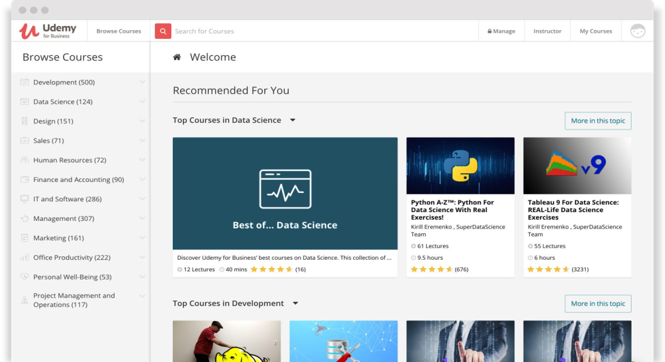
\includegraphics[width= 13 cm]{udemydash.png}
\caption{Udemy Courses}
\end{figure}

\subsection{History}

In 2007, Udemy founder Eren Bali built software for a live virtual classroom while living in Turkey. He saw potential in making the product free for everyone, and moved to Silicon Valley to found a company two years later. The site was launched by Bali, Oktay Caglar and Gagan Biyani in early 2010.

In February 2010, the founders tried to raise venture capital funding, but the idea failed to impress investors and they were rejected 30 times, according to Gagan Biyani. In response to this, they bootstrapped the development of the product and launched Udemy—"The Academy of You"—in May 2010.

Within a few months, 1,000 instructors had created about 2,000 courses, and Udemy had nearly 10,000 registered users. Based on this favorable market reaction, they decided to attempt another round of financing, and raised \$1 million in venture funding by August.

In October 2011, the company raised an additional \$3 million in Series A funding led by Groupon investors Eric Lefkofsky and Brad Keywell, as well as 500 Startups and MHS Capital.

In December 2012, the company raised \$12 million in Series B funding led by Insight Venture Partners, as well as Lightbank Capital, MHS Capital and Learn Capital, bringing Udemy's total funding to \$16 million.

On April 22, 2014, the Wall Street Journal's Digital edition reported that Dennis Yang, Chief Operating Officer of Udemy was named CEO, replacing Eren Bali.

In May 2014, Udemy raised another \$32 million in a Series C funding, led by Norwest Venture Partners, as well as Insight Venture Partners and MHS Capital.

In June 2015, Udemy raised a \$65 million Series D financing round, led by Stripes Group. Now Udemy joined another online learning house Skillsdox Inc of Canada to open up School of Skills in India.

In June 2016, Udemy raised \$60 million from Naspers Ventures as a follow-up to the \$65 million Series D round of financing from June 2015.

On June 1, 2017, Udemy announced that the board of the company has appointed Kevin H. Johnson as its new chief executive officer effective immediately.

\subsection{Platform}

Udemy is a web application and so it can be used cross-platform. A web browser is the only requirement to use Udemy on the desktop. Users can watch the video lectures of their purchased courses in Udemy using the browser. However, it is better to use the mobile applications for using Udemy in mobile devices.

In April 2013, Udemy offered an app for Apple iOS, allowing students to take classes directly from iPhones; The Android version was launched in January 2014. As of January 2014, the iOS app had been downloaded over 1 million times, and 20 percent of Udemy users access their courses via mobile. In July 2016, Udemy expanded their iOS platform to include Apple TV.

\subsection{Conclusion}
Udemy is a leading global marketplace for learning and instruction. By connecting students all over the world to the best instructors, Udemy is helping individuals reach their goals and pursue their dreams. Udemy is the leading global marketplace for teaching and learning, connecting students everywhere to the world’s best instruction anywhere.

Udemy helps organizations of all kinds prepare for the ever-evolving future of work. Their business and technical courses gives companies, governments, and nonprofits the power to develop in-house expertise and satisfy employees’ hunger for learning and development.

Udemy is a great place to get really good courses on most of the topics you ever want to learn. The courses provided are of great quality. But still there are some courses which are of lower quality and could be a waste. Such low quality courses may also occassionally find their way through good quality courses. They need to be filtered out. Udemy is a good place to start learning something new.

\section{DialogFlow}
\subsection{Introduction}

Dialogflow (formerly Api.ai, Speaktoit) is a Google-owned developer of human–computer interaction technologies based on natural language conversations. The company is best known for creating the Assistant (by Speaktoit), a virtual buddy for Android, iOS, and Windows Phone smartphones that performs tasks and answers users' question in a natural language.

Speaktoit has also created a natural language processing engine that incorporates conversation context like dialogue history, location and user preferences.

Chatbots built with DialogFlow are intelligent personal assistants. Dialogflow abstracts out the Natural Language Processing, Machine Learning and other deeper concepts and gives a clean usable user interface to focus on the conversation flow and build bots.

\begin{figure}[h]
\label{ss}    %Figure Label is used
\centering

\includegraphics[width= 6 cm]{dialogflow.jpg}
\caption{Dialogflow}
\end{figure}

\subsection{Overview}

Dialogflow can be used to give our users new ways to interact with the product by building engaging voice and text-based conversational interfaces, such as voice apps and chatbots, powered by AI. It helps us to better connect with users on our website, mobile app, the Google Assistant, Amazon Alexa, Facebook Messenger, and other popular platforms and devices.

Dialogflow (the voice-enabling engine that powers Google Assistant) provides APIs to third-party developers, allowing the addition of voice interfaces to apps based on Android, iOS, HTML5, and Cordova. The SDK's contain {\em voice recognition, natural language understanding, and text-to-speech}. It provides a web interface to build and test conversation scenarios. The platform is based on the natural language processing engine built by Speaktoit for its Assistant application. It also provides support for IoT devices. It provides tools to developers building apps or {\em Actions} for the Google Assistant virtual assistant.\\

\begin{figure}[h]
\label{ss}    %Figure Label is used
\centering
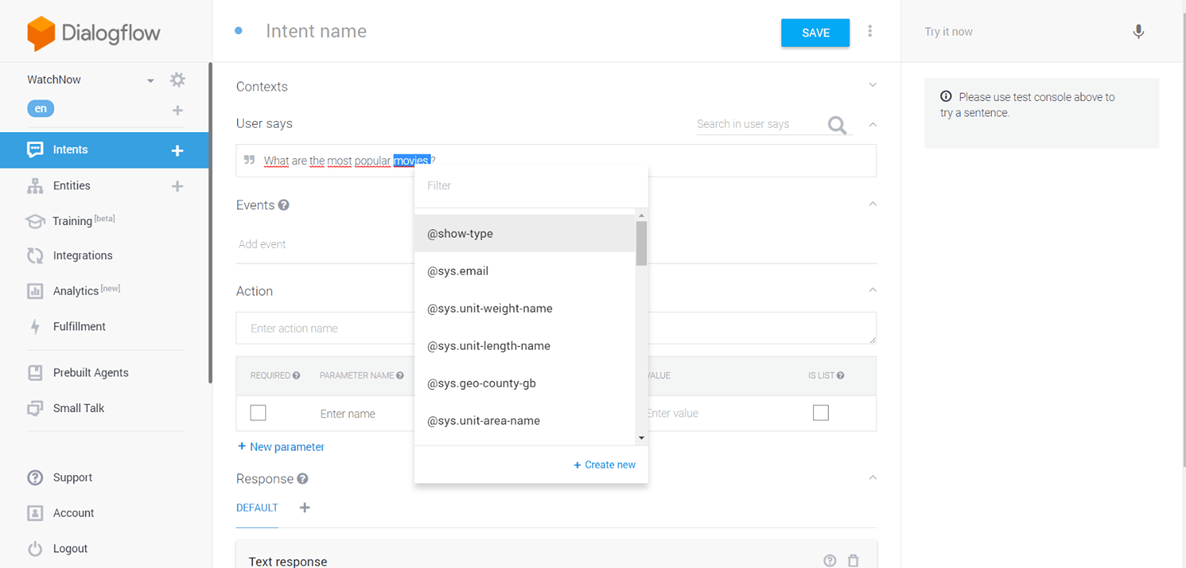
\includegraphics[width= 13 cm, height = 7cm]{dialogflowdash.png}
\caption{Dialogflow Console}
\end{figure}

\subsection{Features}

Voice and conversational interfaces created with Dialogflow works with a wide range of devices including phones, wearables, cars, speakers and other smart devices. 
It supports 14+ languages including Brazilian Portuguese, Chinese, English, Dutch, French, German, Italian, Japanese, Korean, Portuguese, Russian, Spanish and Ukrainian. 
Dialogflow supports an array of services that are relevant to entertainment and hospitality industries. 
Dialogflow also includes an analytics tool that can measure the engagement or session metrics like usage patterns, latency issues, etc.

\subsubsection {Powered By Google}
Dialogflow incorporates Google's machine learning expertise and products such as Google Cloud Speech-to-Text.
\subsubsection {Built on Google}
Dialogflow is backed by Google and runs on Google Cloud Platform, letting you scale to hundreds of millions of users.
\subsubsection {Optimized for the Google Assistant}
Dialogflow is the most widely used tool to build Actions for more than 400M+ Google Assistant devices.
\subsubsection {Multiple Platforms}
Build Actions, Skills, bots, and apps for the Google Assistant, Alexa, Cortana, Facebook Messenger and other platforms your users are on.
\subsubsection {Multiple Devices}
Whether your users are on-the-go or at home, engage with them through wearables, phones, cars, speakers and other smart devices.
\subsubsection {Multiple Languages}
Broaden your reach globally with 20+ supported languages including Spanish, French, and Japanese.



\subsection{History}

In May 2012, Speaktoit received a venture round from Intel Capital. 
In July 2014, Speaktoit closed their Series B funding led by Motorola Solutions Venture Capital with participation from new investor Plug and Play Ventures and existing backers Intel Capital and Alpine Technology Fund.
In September 2014, Speaktoit released api.ai.
Google bought the company in September 2016. 
The organization discontinued the Assistant app on December 15, 2016. 
It was renamed on 10 October 2017 as Dialogflow.

\subsection{Platform}

Dialogflow can be used to develop conversational bots for website, mobile app, the Google Assistant, Amazon Alexa, Facebook Messenger, and other popular platforms and devices. It can also be implemented in apps based on Android, iOS, HTML5, and Cordova.

Other supported integrations are:
\begin{itemize}

\item{Google Assistant}

\item{Facebook Messenger}

\item{Slack}

\item{Kik Messenger}

\item{Line Messenger}

\item{Skype}

\item{Telegram}

\item{Twitter}

\item{Twilio}
\end{itemize}

\subsection{Used by}
Dialogflow is being used my many big players across a wide range of industries. They use Dialogflow to harness the power and reach of conversational experiences with their users and customers. Some of these vendors are :
\begin{itemize}

\item{Comcast}

\item{Domino's}

\item{KLM Royal Dutch Airlines}

\item{Giorgio Armani}

\item{Mercedes-Benz}

\item{The Wall Street Journal}

\item{npr one}
\end{itemize}

\subsection{Conclusion}
Dialogflow is considered to be the best chatbot platform available right now. It's Natural Language Processing is best in class. It is backed by Google's Machine Learning.

Dialogflow offers the Standard Edition for free allowing unlimited text queries and 1000 voice queries per day. The Standard Edition is more than enough for developing a basic chabot.

Dialogflow really takes the hassle out of building a chatbot for our product. It is one of the best in its league.

\chapter{PRODUCT DESIGN}  % Short of the project name

{\em A platform for online learning which brings together interactivity and in-depth knowledge.}


\section{Introduction}

Many online resources are available today to learn coding.But we fail to find out the best mixture of features at one portal. Lack of interactivity and and in-depth training is one of the main problem with this. Virtua teacher provide better solution for this. It is the integration of data analysis and intelligence to the existing online learning platforms so that it can achieve the ability to enable in-depth traing and more interactivity.


\section{ Scope}
Since they lack interactivity many online platforms with large number of enrollements have only 35\% graduation rate. Improving interactivity by providing forums and discussion , virtual classes have proven to increase the productivity rate in the terms of improved through-put and the user also doesn't get bored overtime.Intelligence and personalisation improves the interactivity 10times better than the existing interacting factors. Voice enabled feedback machines is showing up everywhere and hoped to be common in the future technologies, since this project includes a chatbot which can also be enabled with voice output

\section{ Software Development Life Cycle}

The System Development Life Cycle framework provides system designers and developers to follow a sequence of activities. It consists of a set of steps or phases in which each phase of the SDLC uses the results of the previous one.
A Systems Development Life Cycle (SDLC) adheres to important phases that are essential for developers, such as planning, analysis, designs and implementation and are explained in the section below. A number of system development life cycle (SDLC) models have been created: waterfall, fountain and spiral build and fix, rapid prototyping, incremental, and synchronize and stabilize. The oldest of these, and the best known, is the waterfall model: a sequence of stages in which the output of each stage becomes the input for the next.These stages can be characterized and divided up in different ways, including the following:

1.Project planning, feasibility study: Establishes a high-level view of the intended project and determines its goals.

2. Systems analysis, requirements definition: Refines project goals into defined functions and operation of the intended application. Analyzes end-user information needs.

3. Systems design: Describes desired features and operations in detail, including screen layouts, business rules, process diagrams, pseudo code and other documentation.

4. Implementation: The real code is written here.

5. Integration and testing: Brings all the pieces together into a special testing environment, then checks for errors, bugs and interoperability.

6. Acceptance, installation, deployment: The final stage of initial development, where the software is put into production and runs actual business.

7. Maintenance: What happens during the rest of the software's life: changes, correction, additions and moves to a different computing platform and more? This, the least glamorous and perhaps most important step of all, goes on seemingly forever.

The following figure is a graphical representation of the various stages of a typical SDLC.
\begin{figure}[h]
	\label{ss}    %Figure Label is used
	\centering
	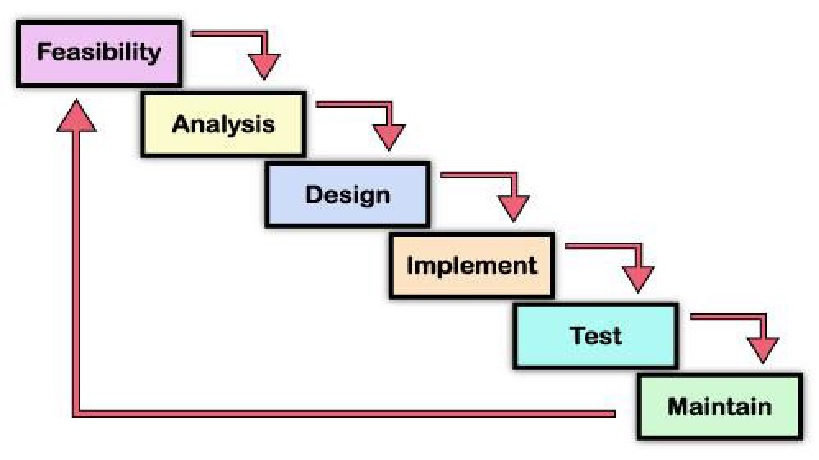
\includegraphics[width= 8 cm]{sdlc.jpg}
	\caption{ Software Development Life Cycle}
\end{figure}
\section{Feasibility Study}
A feasibility analysis usually involves a thorough assessment of the operational (need), financial and technical aspects of a proposal. Feasibility study is the test of the system proposal made to identify whether the user needs may be satisfied using the current software and hardware technologies, whether the system will be cost effective from a business point of view and whether it can be developed with the given budgetary constraints. A feasibility study should be relatively cheap and done at the earliest possible time. Depending on the study, the decision is made whether to go ahead with a more detailed analysis. When a new project is proposed, it normally goes through feasibility assessment. Feasibility study is carried out to determine whether the proposed system is possible to develop with available resources and what should be the cost consideration. Facts considered in the feasibility analysis were-

\begin{itemize}
\item{Technical Feasibility}

	\item{Economic Feasibility}

	\item{Behavioral Feasibility}
\end{itemize}

\subsection{Technical Feasibility }
Technical feasibility includes whether the technology is available in the market for development and its availability. The assessment of technical feasibility must be based on an outline design of system requirements in terms of input, output, files, programs and procedures.

This can be qualified in terms of volumes of data, trends, frequency of updating, cycles of activity etc., in order to give an introduction of technical system.
\subsection{Economic Feasibility}
This feasibility study present tangible and intangible benefits from the project by comparing the development and operational cost. The technique of cost benefit analysis is often used as a basis for assessing economic feasibility. This system needs some more initial investment than the existing system, but it can be justifiable that it will improve quality of service.

Thus feasibility study should center along the following points:

1. Improvement resulting over the existing method in terms of accuracy, timeliness.

2. Cost comparison

3. Estimate on the life expectancy of the hardware.
\subsection{Behavioral/Operational Feasibility}
This analysis involves how it will work when it is installed and the assessment of political and managerial environment in which it is implemented. People are inherently resistant to change and computers have been known to facilitate change. The new proposed system is very much useful to the users and therefore it will accept broad audience from around the world.


\section{System Analysis}
To design and build an application that provides users to watch and attend online courses. The application also hosts a push notification module and a chatbot module.  It uses following environment and tools for the development of the project application. All the information is provided below.

We will discuss about the Android architected in the form of a software stack comprising applications, an operating system, run-time environment, middleware, services and libraries. This architecture can, perhaps, best be represented visually. Each layer of the stack, and the corresponding elements within each layer, are tightly integrated and carefully tuned to provide the optimal application development and execution environment for mobile devices.

All these phases are cascaded to each other in which progress is seen as flowing steadily downwards (like a waterfall) through the phases. The next phase is started only after the defined set of goals are achieved for previous phase and it is signed off, so the name "Waterfall Model". In this model, phases do not overlap.




\subsection{Android Studio and Android SDK }

Android Studio is the official IDE for Android app development, based on IntelliJ IDEA. On top of IntelliJ's powerful code editor and developer tools, Android Studio offers even more features that enhance your productivity when building Android apps, such as:
\begin{itemize}

\item{A flexible Gradle-based build system}

	\item{Build variants and multiple APK file generation}

	\item{Code templates to help you build common app features}

\item{A rich layout editor with support for drag and drop theme editing}

\item{ Lint tools to catch performance, usability, version compatibility, and other problems}

\item{Code shrinking with ProGuard and resource shrinking with Gradle}

\item{Built-in support for Google Cloud Platform, making it easy to integrate Google Cloud Messaging and App Engine}
\end{itemize}


\subsection{SQLite Database}

SQLite is a relational database management system contained in a C programming library. In contrast to many other database management systems, SQLite is not a client–server database engine. Rather, it is embedded into the end program. SQLite is ACID-compliant and implements most of the SQL standard, using a dynamically and weakly typed SQL syntax that does not guarantee the domain integrity.

SQLite is a popular choice as embedded database software for local/client storage in application software such as web browsers. It is arguably the most widely deployed database engine, as it is used today by several widespread browsers, operating systems, and embedded systems, among others. SQLite has bindings to many programming languages.
\subsection{Push Notification Module}
A push notification is a message that pops up on a mobile device. App publishers can send them at any time; users don't have to be in the app or using their devices to receive them. They can do a lot of things; for example, they can show the latest sports scores, get a user to take an action, such as downloading a coupon, or let a user know about an event, such as a flash sale.

Push notifications look like SMS text messages and mobile alerts, but they only reach users who have installed your app. Each mobile platform has support for push notifications — iOS, Android, Fire OS, Windows and BlackBerry all have their own services.

\subsubsection{Actors in Push Notifications:}
\begin{itemize}

\item{Operating system push notification service (OSPNS): Each mobile operating system (OS), including iOS, Android, Fire OS, Windows, and BlackBerry, has its own service.}

\item{App publisher: The app publisher enables their app with an OSPNS. Then, the publisher uploads the app to the app store.}

\item{Client app: This is an OS-specific app, installed on a user's device. It receives incoming notifications.}

\end{itemize}

\subsubsection{Implementation of push notifications:}
\begin{itemize}

\item{The app publisher registers with the OS \em\bf{ push notification service.}}

\item{The OS service provides an application programming interface (API) to the app publisher.}

\item{The app publisher adds the SDK to the app. The SDK is a code library specific to the OS' push notification service.}

\end{itemize}

\subsubsection{Sending Push Notifications:}
\begin{itemize}

\item{The app publisher composes a manual message through a message composer user interface. Or, the publisher sets up an automated message to be sent via the API.}

\item{The publisher defines the audience to whom the push notification will be sent.}

\item{The publisher determines whether the message should be sent immediately or scheduled.}

\end{itemize}


\subsection{Chatbot Module}

A chatbot is a computer program or an artificial intelligence which conducts a conversation via auditory or textual methods. Such programs are often designed to convincingly simulate how a human would behave as a conversational partner, thereby passing the Turing test. Chatbots are typically used in dialog systems for various practical purposes including customer service or information acquisition. Some chatterbots use sophisticated natural language processing systems, but many simpler systems scan for keywords within the input, then pull a reply with the most matching keywords, or the most similar wording pattern, from a database.

Many companies' chatbots run on messaging apps like Facebook Messenger (since 2016), WeChat (since 2013),[15] WhatsApp, LiveChat, Kik, Slack, Line, Telegram, or simply via SMS. They are used for B2C customer service, sales and marketing.[16]

\subsubsection{Developing a Chatbot}
The process of creating a chatbot follows a pattern similar to the development of a web page or a mobile app. It can be divided into Design, Building, Analytics and Maintenance.\\

{\bf Design}\\
The chatbot design is the process that defines the interaction between the user and the chatbot. The chatbot designer will define the chatbot personality, the questions that will be asked to the users, and the overall interaction. It can be viewed as a subset of the conversational design. In order to speed up this process, designers can use dedicated chatbot design tools, that allow for immediate preview, team collaboration and video export. An important part of the chatbot design is also centered around user testing. User testing can be performed following the same principles that guide the user testing of graphical interfaces

{\bf Building}\\
The process of building a chatbot can be divided into two main tasks: understanding the user's intent and producing the correct answer. The first task involves understanding the user input. In order to properly understand a user input in a free text form, a Natural Language Processing Engine can be used. The second task may involve different approaches depending on the type of the response that the chatbot will generate.

{\bf Analytics}\\
The usage of the chatbot can be monitored in order to spot potential flaws or problems. It can also provide useful insights that can improve the final user experience.

{\bf Maintenance}\\
To keep chatbots up to speed with changing company products and services, traditional chatbot development platforms require ongoing maintenance. This can either be in the form of an ongoing service provider or for larger enterprises in the form of an in-house chatbot training team. To eliminate these costs, some startups are experimenting with Artificial Intelligence to develop self-learning chatbots, particularly in Customer Service applications.

{\bf Chatbot development platforms}\\
The process of building, testing and deploying chatbots can be done on cloud based chatbot development platforms offered by cloud Platform as a Service (PaaS) providers such as Oracle Cloud Platform, SnatchBot and IBM Watson. Dialogflow by Google is one of the best such platforms in existence. These cloud platforms provide Natural Language Processing, Artificial Intelligence and Mobile Backend as a Service for chatbot development.

\begin{figure}[h]
	\label{ss}    %Figure Label is used
	\centering
	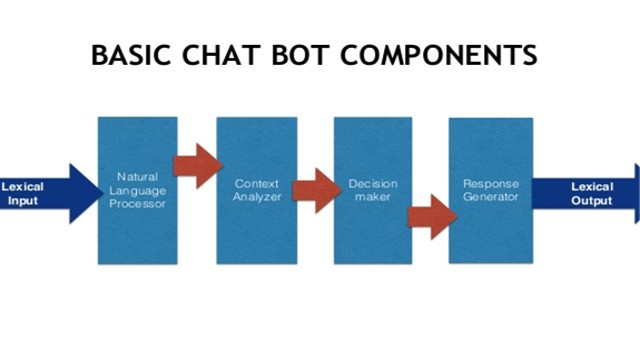
\includegraphics[width= 9 cm]{chatbotdiagram.jpg}
	\caption{ Chatbot Components}
\end{figure}

\section{System Requirement Specification}


\subsubsection{Hardware requirements:}

System Processor : Pentium P4\\
Mobile Processor : 1GHz or higher\\
Motherboard : Genuine Intel\\
RAM : 1 GB or higher\\ Memory : 200 MB or higher

\subsubsection{Software requirements:}


Technology Used : Android 4.1 or higher\\
IDE : Android Studio\\
Emulators : Micro emulator 555\\
Plug-in : ADT plug-in\\
Back-End : php, SQLite\\
Front-End : Android SDK\\

\subsection{Web Server Requirements:}
The Web Server Subsystem shall use insert-db.php and get.php to make HTTP requests/ responses to Web Application Subsystem and the Database Subsystem.

\subsection{Device Permission Requirement}
Application requires some permissions in order to establish a connection. These must have mention in Android manifest le. These permissions are:

\begin{itemize}

\item{Internet

This permission is required for to access the internet using the application.}

\item{ACCESS\_COARSE\_LOCATION

This permission is required for tracking the location of the user to personalize and determine sending push notifications.}

\item{RECORD\_AUDIO

This permission is required to accept voice input from the user for the chatbot module.}


\end{itemize}

\section{System Design}
This part describes features, fragments, classes, architecture and the application itself by providing necessary information of major components. First, an overall information is given along with project's components and classes. Subsequently, the architecture details of the application is discussed.

\subsection{Components}
In order to provide a detailed view concerning system mechanism, project can be grouped in three segments. These are User Authentication, Course Catalog, Lecture Video Player, Push Notification module, Chatbot Module.

\subsubsection{User Authentication}

User Authentication component includes the Login/Signup form through which the user can login or signup to the application. The Login and Signup forms will be easily switchable without much hassle. Both forms will be available in the same page as switchable tabs. Users will also have the option to login with their Social Media accounts such as Google, Facebook, Twitter, GitHub. OAuth authentication will be implemented for this.

\subsubsection{Course Catalog}

Course catalog is a simple User Interface listing all the courses available and Selection of a course for the user to enroll. Course Catalog has a simple and intuitive design which provides a First Glance view of all courses available. First Glance view will display all the courses as tiles in which the Course Name, Course Description, Course Rating, No. of enrolled students, Preview Video and Price.

\subsubsection{Lecture Video Player}

When a user opts to watch the lecture videos of a course, he/she will be taken to the Lecture Video Player. Lecture Video Player is a video playback module for lecture video playback. It will have an intuitive design with several useful features which provides a rich user experience. It will have options to Play, Pause, Stop and Seek the video. User will be able to select the video quality from among 3-4 quality options. User will also have the option to select the playback speed from among 4-5 speed options. An option to set Autoplay on or off will be available. If Autoplay is set, the subsequent lectures in the lesson will automatically start playing when previous video completes. All video lectures in the lesson will be easily viewable and selectable in the player.

\subsubsection{Push Notification Module}
To implement the push notification module in the application, we've used the {\em OneSignal} push notification service available online. OneSignal provides a simple interface to push notifications and email, letting content creators focus on quality user engagement instead of complex implementation. They provide High volume, cross platform push notification delivery. OneSignal provides push notification services for Android applications as well.

We require an account at OneSignal to use their service. The application needs to be registered with OneSignal. We create a new app in OneSignal in the account dashboard. OneSignal App ID needs to be noted. This App ID is to be included in a code snippet in the Android Application source code. This code snippet is used to initialise the OneSignal service in our Android app and it is made available in the OneSignal documentation. Notification features like icon and email are also configured.

To send a new push notification from OneSignal, we use the {\em New Push} option available in the OneSignal dashboard. We need to select the {\em Audience}, {\em Specify message}, {\em Select Platforms}, {\em Select Icon}. {\em Additional Data} in the form of {\em Key-Value pairs} also need to be specified if any. {\em Messages can also be scheduled} by selecting the date and time.

\subsubsection{ChatBot Module}
We've used Google's {\em Dialogflow} to implement the chatbot or conversational interface in our Android App. Dialogflow provides a rich experience and robust results in developing a powerful conversational interface.

Implementing a Dialogflow interface in our Android App:
\begin{enumerate}
  \item Login to the Dialogflow console using Google Account.
  \item Create a new agent in 
  \item Etc.
\end{enumerate}

\subsection{Block Diagram}
\begin{figure}[h]
	\label{ss}    %Figure Label is used
	\centering
	\includegraphics[width= 13 cm]{dfd.png}
	\caption{System Block Diagram}
\end{figure}



user can use the app to view the courses and syllabus and enroll for the same, and learn the enrolled courses and complete the course certifications , he/she can use the chatbot to ask doubts or post in forum using the app.The instructors can use the app to create courses with required resources , Answer the queries posted in forum by the users enrolled his or her course or other courses. He can view his currently enrolled users and their status of learning.




\newpage
\subsection{Data Flow Diagram}
The DFD was first developed by Larry Constiane as a way of expressing system in a graphical form. A DFD, also known as Bubble Chart, has a purpose of clarifying system requirement and identifying major transformation that will become the programs in the system design.
\begin{figure}[h]
	\label{ss}    %Figure Label is used
	\centering
	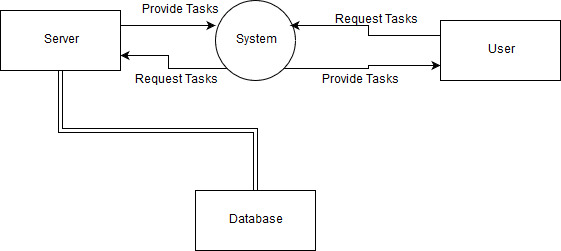
\includegraphics[width= 13 cm]{dfd3.jpg}
	\caption{Data Flow Diagram}
\end{figure}



\newpage
\subsection{Level DFD}



\begin{figure}[h]
	\label{ss}    %Figure Label is used
	\centering

	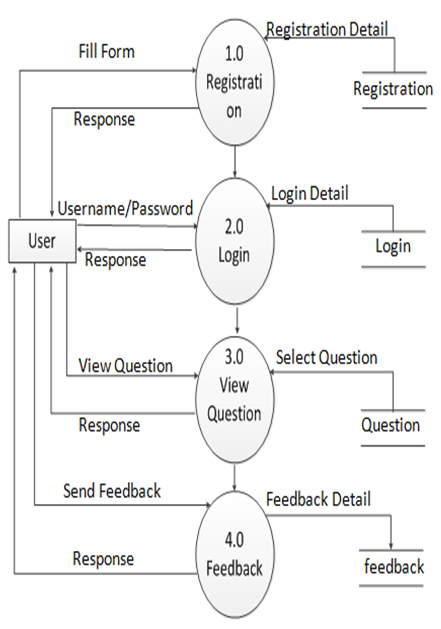
\includegraphics[width= 11 cm]{user.png}
	\caption{user level DFD}
\end{figure}
\newpage
\begin{figure}[h]
	\label{ss}    %Figure Label is used
	\centering
	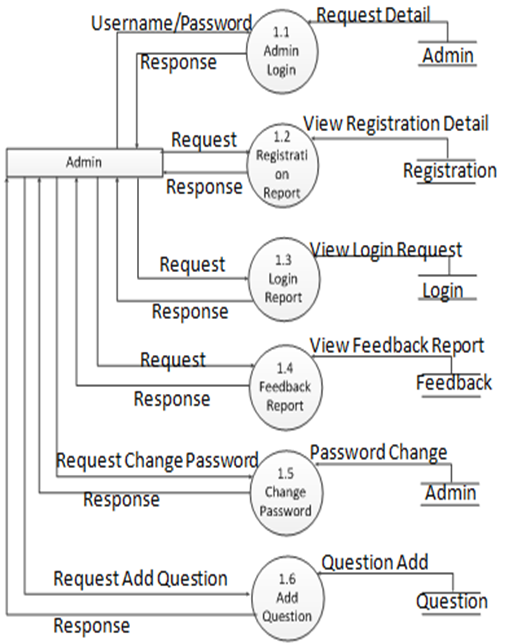
\includegraphics[width= 13 cm]{admin.png}
	\caption{First Level DFD For Server}
\end{figure}
\newpage
\begin{figure}[h]
	\label{ss}    %Figure Label is used
	\centering
	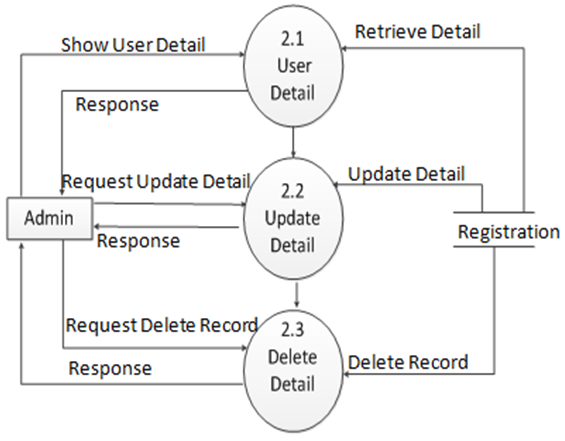
\includegraphics[width= 13 cm]{admin2.png}
	\caption{First Level DFD For Server}
\end{figure}






\subsection{Database Design}
\begin{figure}[h]
	\label{ss}    %Figure Label is used
	\centering
	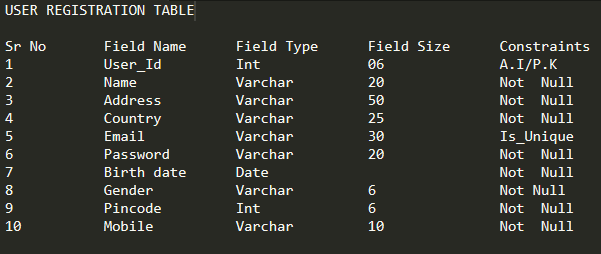
\includegraphics[width= 11 cm]{regtable.png}
	\caption{User Registration Table}
\end{figure}

\newpage

\begin{figure}[h]
	\label{ss}    %Figure Label is used
	\centering
	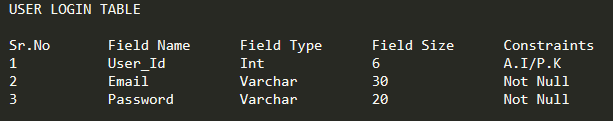
\includegraphics[width= 13 cm]{ulogin.png}
	\caption{User login Table}
\end{figure}

\begin{figure}[h]
	\label{ss}    %Figure Label is used
	\centering
	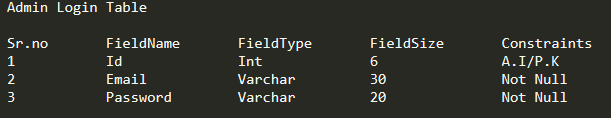
\includegraphics[width= 13 cm]{alogin.png}
	\caption{Admin login Table}
\end{figure}
\begin{figure}[h]
	\label{ss}    %Figure Label is used
	\centering
	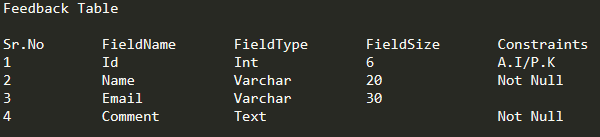
\includegraphics[width= 13 cm]{feedback.png}
	\caption{Feedback Table}
\end{figure}


\newpage
\section{Implementation}

Project is designed in four parts where each part is responsible for different aspects. Essentially, Login Activity handles session to which the user is directed to , to a student profile or an instructor profile. It also consists standard Android life cycle methods.
\subsection{Overview}
User must be directed to his corresponding session using previously logged in data which is stored in shared preferences.App must always run a service in background and ignored battery consumption warning to push notifications properly.
Using this application:-
\begin{itemize}	
\item{The user must be able to learn without being stressed out.}

\item{They can be stayed in focus for more hours due to interactiveness of the application.}

\item{All instructors must provide the course in mentioned standards like possible queries from an user and its answer , proper resources and lessons divided as tasks. This helps to maintain the homogenity among the courses and because of this user becomes comfortable with the system after some time.}

\item{Users can use chatbots to clarify their doubts regarding the tasks than posting it in a forum andwaiting for someoneto reply and others to validate is reply, If the query is not in the database of chat bot , chatbot learns the new query  and wait for the instructor to provide its answer.}

\end{itemize}




\subsection{Activity Diagram}
Activity diagramis basically a flow chart to represent the flow form oneactivityto anotheractivity. Theactivity can be described as an operation of the system. So the control flow is drawn from one operation to another. This flow can be sequential, branched or concurrent.
\begin{figure}[h]
	\label{ss}    %Figure Label is used
	\centering
	\includegraphics[width= 13 cm]{flow.png}
	\caption{Activity Diagram}
\end{figure}

\subsection{Use-Case Diagram}

A use case diagram at its simplest is a representation of a user's interaction with the system that shows the relationship between the user and the different use cases in which the user is involved. A use case diagram can identify the different types of users of a system and the different use cases and will often be accompanied by other types of diagrams as well.

\begin{figure}[h]
	\label{ss}    %Figure Label is used
	\centering
	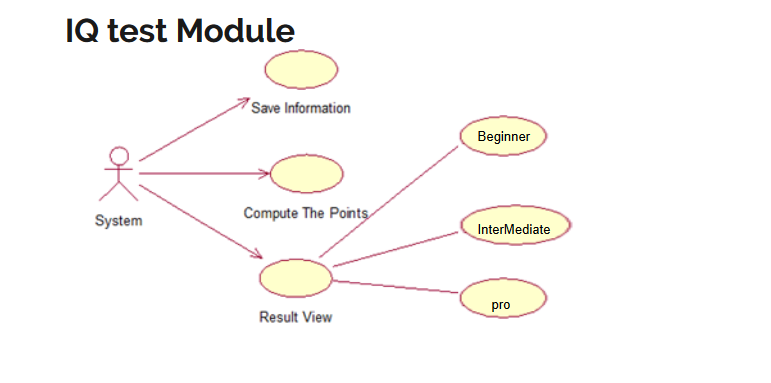
\includegraphics[width= 13 cm]{iqusecase.png}
	\caption{Use-Case Diagram}
\end{figure}
\newpage
\begin{figure}[h]
	\label{ss}    %Figure Label is used
	\centering
	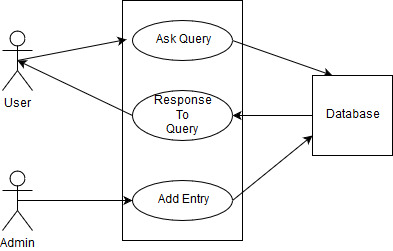
\includegraphics[width= 13 cm]{chatbot.jpg}
	\caption{Use-Case Diagram}
\end{figure}
\chapter{Testing}
{\em Testing is a process, which reveals errors in the program. It is the major quality measure employed during software development. During software development. During testing, the program is executed with a set of test cases and the output of the program for the test cases is evaluated to determine if the program is performing as it is expected to perform.}
\section {TESTING STRATEGIES}
In order to make sure that the system does not have errors, the different levels of testing strategies that are applied at differing phases of software development are:
\subsection{Unit Testing:}
Unit Testing is done on individual modules as they are completed and become executable. It is confined only to the designer's requirements.

Each module can be tested using the following two Strategies:

Black Box Testing:

In this strategy some test cases are generated as input conditions that fully execute all functional requirements for the program. This testing has been uses to find errors in the following categories:
\begin{itemize}

\item{ Incorrect or missing functions.}

	\item{Interface errors}

	\item{Errors in data structure or external database access}
\item{Initialization and termination errors}
\item{Performance errors}

\end{itemize}
In this testing only the output is checked for correctness. The logical flow of the data is not checked.
White Box testing:
In this the test cases are generated on the logic of each module by drawing flow graphs of that module and logical decisions are tested on all the cases. It has been uses to generate the test cases in the following cases:
\begin{itemize}

\item{Guarantee that all independent paths have been executed.}

	\item{Execute all logical decisions on their true and false Sides.}

	\item{Execute all loops at their boundaries and within their operational bounds}

\item{Execute internal data structures to ensure their validity}

\end{itemize}
\subsection{Integrating Testing:}
Integration testing ensures that software and subsystems work together a whole. It tests the
interface of all the modules to make sure that the modules behave properly when integrated
together.
\subsection{System Testing:}
Involves in-house testing of the entire system before delivery to the user. Its aim is to satisfy
the user the system meets all requirements of the client's specifications.
\subsection{Acceptance Testing:}
It is a pre-delivery testing in which entire system is tested at client's site on real world data
to find errors.
\section{Test Approach}
Testing can be done in two ways:
\subsection{Bottom up Aproach:}
Testing can be performed starting from smallest and lowest level modules and proceeding one at a time. For each module in bottom up testing a short program executes the module and provides the needed data so that the module is asked to perform the way it will when embedded within the larger system. When bottom level modules are tested attention turns to those on the next level that use the lower level ones they are tested individually and then linked with the previously examined lower level modules.
\subsection{Top down Aproach:}
This type of testing starts from upper level modules. Since the detailed activities usually performed in the lower level routines are not provided stubs are written. A stub is a module shell called by upper level module and that when reached properly will return a message to the calling module indicating that proper interaction occurred. No attempt is made to verify the correctness of the lower level module.
\section{Validation and Verification:}
The system has been tested and implemented successfully and thus ensured that all the requirements as listed in the software requirements specification are completely fulfilled. In case of erroneous input corresponding error messages are displayed.

In software project management, software testing, and software engineering, verification and validation (VandV) is the process of checking that a software system meets specifications and that it fulfills its intended purpose. It may also be referred to as software quality control. It is normally the responsibility of software testers as part of the software development lifecycle.

Validation checks that the product design satisfies or fits the intended use (high-level
checking), i.e., the software meets the user requirements. This is done through dynamic
testing and other forms of review.

Verification and validation are not the same thing, although they are often confused. Boehm
succinctly expressed the difference between

Verification: Are we building the product right?

Validation: Are we building the right product?

According to the Capability Maturity Model (CMMI-SW v1.1),
Software Verification: The process of evaluating software to determine whether the products
of a given development phase satisfy the conditions imposed at the start of that phase[IEEESTD-
610].

Software Validation: The process of evaluating software during or at the end of the
development process to determine whether it satisfies specified requirements[IEEE-STD-
610].

In other words, software verification is ensuring that the product has been built according to
the requirements and design specifications, while software validation ensures that the
product actually meets the user's needs, and that the specifications were correct in the first
place. Software verification ensures that "you built it right" Software validation ensures that
"you built the right thing". Software validation confirms that the product, as provided, will
fulfill its intended use.

From testing perspective:

Fault – wrong or missing function in the code.

Failure – the manifestation of a fault during execution.

Malfunction – according to its specification the system does not meet its specified
functionality.

\chapter{Future Scope}
\begin{itemize}	
\item{Data of the person is collected in and out of the course. The personality of the person can be
recognised by analysing his/her chats.}

\item{Push notifications and Chatbot messages may be modulated based on the personality of the user.}

\item{Voice output for the chatbots which are more human are expected to come in the future. The voice modulations from Google Duplex which seems more human could be implemented if possible.}
\end{itemize}

\chapter{Conclusion}
Online resources to learn coding lack either interactivity or pace and in-depth training. Many online resources are available today to learn coding. But we fail to find the best mixture of features at one portal. We developed an online learning platform which provides in-depth knowledge and higher level of interactivity. We included a chatbot module and push notifications to provide better interactivity. 
By this project we were able to bring together interactivity and in-depth training into a single learning platform. We put forward a better solution of a coding resource which brings together the best of existing solutions while improving and adding to it. Much more improvements can be introduced into our proposal to make our application more feasible.

%%%%%%%%%%%%%%%%%%%%%%%%%%%%%%%%
%%%%%%%%%%%%%%%%%%%%%%%%%%%%%%%%
%%%%%%%%%%%%%%%%%%%%%%%%%%%%%%%%
\clearpage
%%%%%%%%%%%%%%%%%%%%%%%%%%%%%%%%


%%%%%%%%%%%%%%%%%%%%%%%%%%%%%%%%%%%%
%%%%%%%%%%%%%%%%%%%%%%%%%%%%%%%%%%%%
%%
%%          Bibliography 
%%
%%%%%%%%%%%%%%%%%%%%%%%%%%%%%%%%%%%%
%%%%%%%%%%%%%%%%%%%%%%%%%%%%%%%%%%%%

\clearpage
\addcontentsline{toc}{chapter}{\quad BIBLIOGRAPHY}
\begin{thebibliography}{99}
	%%%%%%%%%%%%%%%%%%%%%%%%%%%%%%%%%%%%
	%%
	%%          Add Bibliography from below, here 3 eg are there
	%%	    If u need to add more bib  use \bibitem   command again & again
	%%
	%%%%%%%%%%%%%%%%%%%%%%%%%%%%%%%%%%%%
	
\bibitem{a}https://en.wikipedia.org/wiki/Codecademy
\bibitem{b}https://www.codecademy.com/
\bibitem{c}https://techcrunch.com/2011/12/22/codecademy-launches-labs-a-web-based-code-editor/
\bibitem{d}https://en.wikipedia.org/wiki/Udemy
\bibitem{e}https://about.udemy.com
\bibitem{f}https://codeburst.io/2-how-assistant-work-introduction-to-dialogflow-319a72ba2db
\bibitem{g}https://medium.com/swlh/how-to-build-a-chatbot-with-dialog-flow-chapter-1-introduction-ab880c348b5
\bibitem{h}https://www.margo-group.com/en/news/a-brief-introduction-to-chatbots-with-dialogflow/your-go-to-map-app.html
\bibitem{i}https://dialogflow.com
\bibitem{j}https://dialogflow.com/docs/integrations

	
	
	








	
\end{thebibliography}



%%%%%%%%%%%%%%%%%%%%%%%%%%%%%%%%%%%%%
%%%%%%%%%%%%%%%%%%%%%%%%%%%%%%%%%%%%%
\clearpage




%%%%%%%%%%%%%%%%%%%%%%%%%%%%%%%%%%%%%
%%%%%%%%%%%%%%%%%%%%%%%%%%%%%%%%%%%%%
%
%   Hi, All
%   Arun Xavier, VAST Thrissur
%
%   for more  Visit my Page - http://arunxeee.blogspot.in/
%
%%%%%%%%%%%%%%%%%%%%%%%%%%%%%%%%%%%%
%%%%%%%%%%%%%%%%%%%%%%%%%%%%%%%%%%%%

%
\end{spacing}
\newpage
\thispagestyle{empty}
\vspace*{\fill}
\begin{flushright}

\includegraphics[width=2.5 cm]{VidyaLogo.JPG}\\[.2 cm]
{\Large \bf \rm  Department of \vdept\ }\\
{\large \rm Vidya Academy of Science \& Technology\\
Thalakkottukara, Thrissur - 680 501\\
({\tt http://www.vidyaacademy.ac.in})}
\end{flushright}

%
\end{document}